\chapter{Results}
\label{chapter:results}

\section{Uncertainties}
\label{sec:uncertainties}

\subsection{Statistical Uncertainties}
\label{ssec:stat_uncertainty}

The statistical uncertainties due to the number of data events are propagated
through the unfolding method, as discussed in
\SEC~\ref{ssec:unfolding_statistical_uncertainties}. This uncertainty is
generally around 0.3\% for both the normalized and absolute cross section
measurement, but reaches 1.2\% in the highest \phistar bins. It is one of the
dominant uncertainties for the normalized cross section measurements.

\subsection{Electron Angular Position Uncertainty}

Since \phistar depends on the angles between the two electrons, it is sensitive
to mismeasurement of these angles. As discussed in
\SEC~\ref{sec:electron_reconstruction}, the position of a reconstructed
electron comes from the tracker, and therefore misalignment of the tracker
would lead to a systematic uncertainty on the angle measurement. The magnitude
of this systematic is estimated by using the position of the ECAL supercluster
associated with the electron to calculate the electron's position instead of
using the track. The new supercluster-only position is then used to calculate a
new \phistarSC that does not depend on the alignment of the tracker.

The position of the supercluster does not take into account the amount the
bending of the electron due to the magnetic field. While $\eta$ is unchanged by
the pretense of the field, $\phi$ is changed. A correction is applied to $\phi$
to find the angle at the interaction point, $\phizero$, based on the angle of
the supercluster, $\phisc$. This correction is given by
\EQ~\ref{eq:b_field_correction} where $q$ is the charge of the electron, \pt is
the transverse momentum of the electron, $B$ is the magnitude of the magnetic
field, and \Reffective is the effective radius of ECAL as a function of $\eta$
and $\theta$ as given in \EQ~\ref{eq:effective_radius}. The charge and momentum
come from the electron matched to the supercluster, and although they are
determined in combination with the tracker, they are far less susceptible to
the small scale misalignments of the tracker that we are considering.

\begin{equation}\label{eq:b_field_correction}
    \sin \left( \phisc - \phizero \right)
    =
    - \Reffective \frac{q B}{2 \pt}
\end{equation}

\begin{equation}\label{eq:effective_radius}
    \Reffective
    =
    \left\{
        \begin{array}{ll}
            1.29 \meters & \text{if } |\eta| < 1.4442 \\
            3.14 \meters \times \tan \left(\coord{\theta}\right) & \text{otherwise}
        \end{array}
    \right.
\end{equation}

The resulting \phistarSC distribution is compatible within statistical
uncertainties with the \phistar distribution and so no systematic uncertainty
is assigned for the angular position.

\TODO{Plot of \phistar vs \phistarSC?}

\subsection{Uncertainty from Four Vector Corrections}

The \mee distribution in the \MADGRAPH signal MC sample does not precisely
match the distribution in data, as seen in \FIG~\ref{fig:z_mass}. This
discrepancy remains even after applying the various energy and momentum
corrections to the electrons. In order to determine what effect this has on the
final measurement, the \MADGRAPH signal MC sample is reweighted to remove this
difference. The ratio between the nominal \phistar value and the value derived
after this reweighting is shown in \FIG~\ref{fig:z_mass_reweighted}. The
circular points show the ratio of the reconstructed \phistar distributions,
while the square points show the ratio of the generated \phistar distributions.
The errors are binomial. Most of the points are consistent with \num{1}, and so
systematic uncertainty is assigned for this disagreement.

\begin{figure}[!htbp]
    \centering
    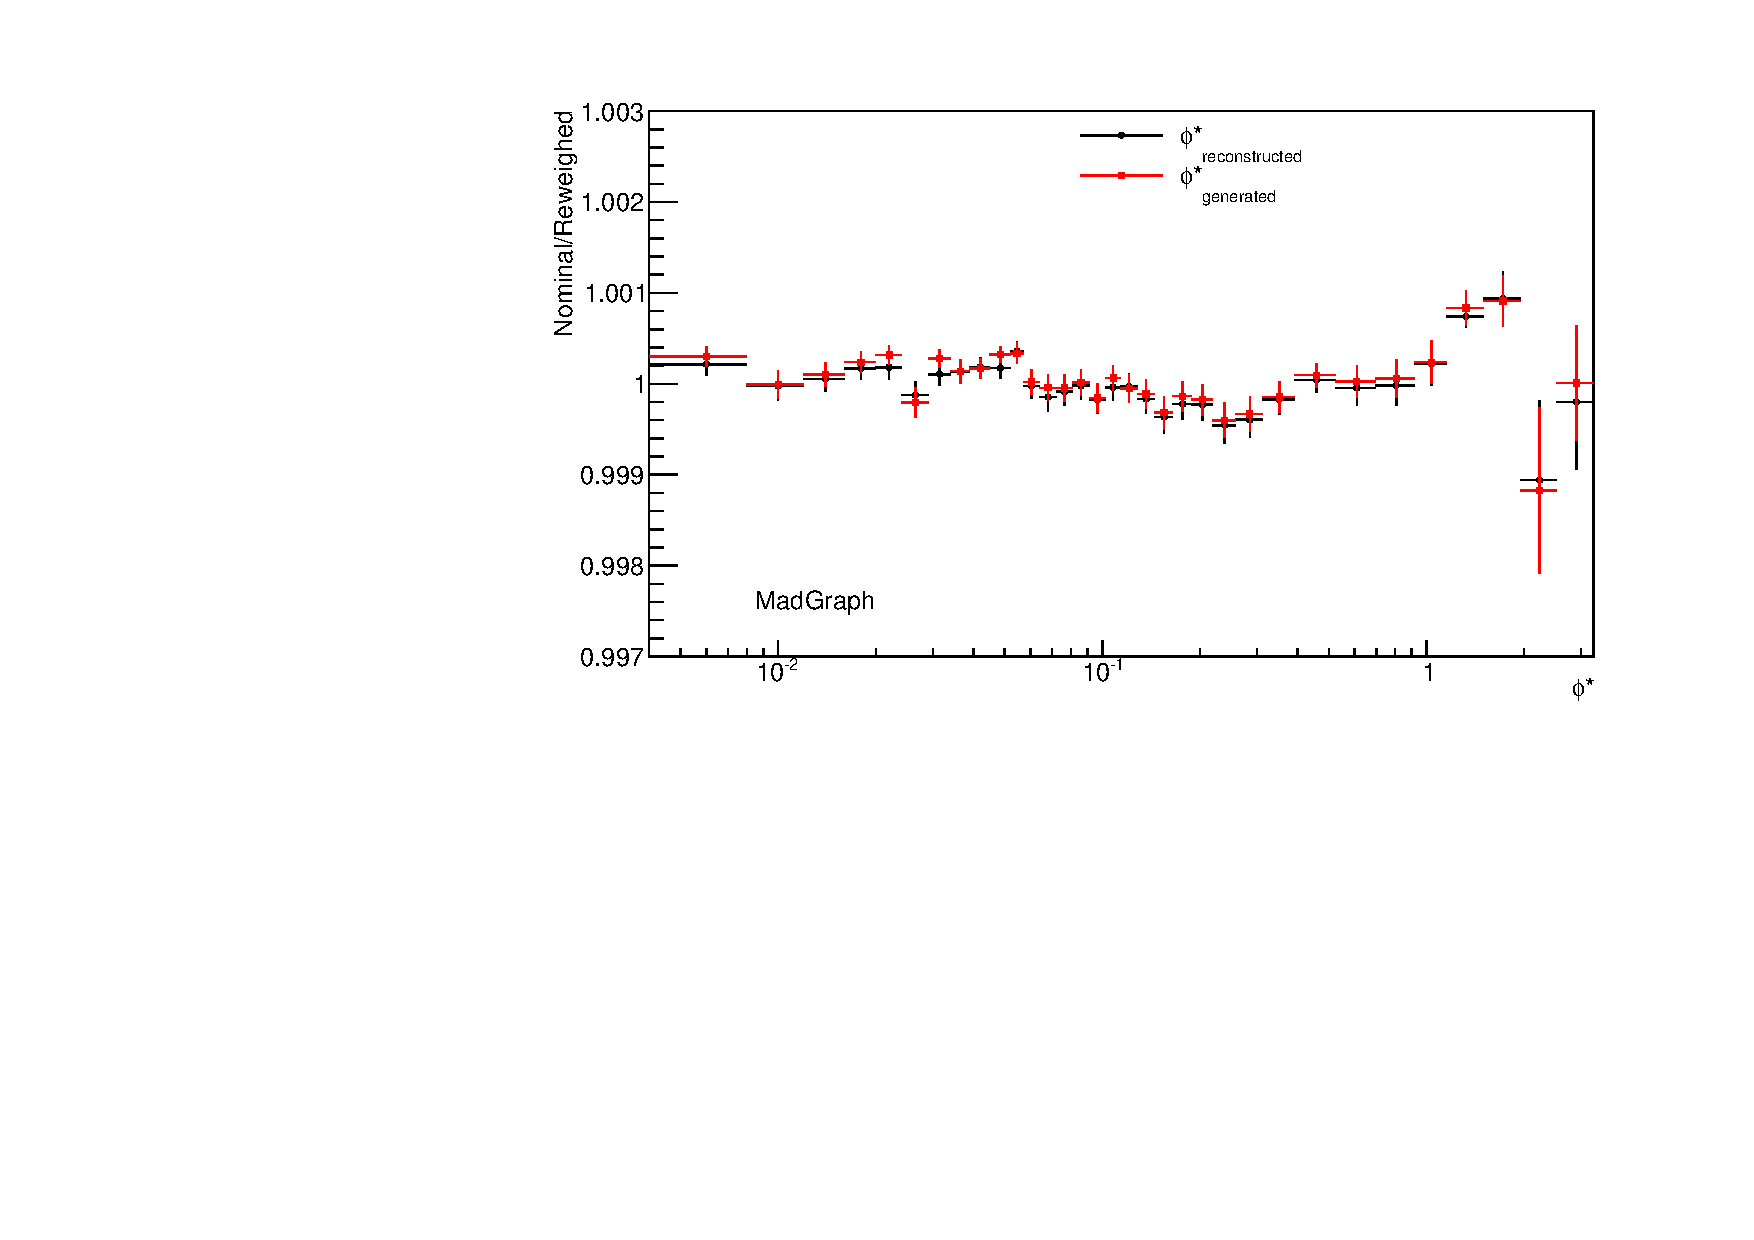
\includegraphics[width=\textwidth]{figures/ZMass_reweighed.pdf}
    \caption[
        The ratio of \phistar in \MADGRAPH before and after reweighting to
        remove the differnce in the \mee distribution between MC and data.
    ]{
        The ratio of \phistar in \MADGRAPH before and after reweighting to
        remove the difference in the \mee distribution between MC and data seen
        in \FIG~\ref{fig:z_mass}. The circular points are this ratio in the
        reconstructed quantity, while the square points are this ratio in the
        generated quantity. The uncertainties are binomial.
    }
    \label{fig:z_mass_reweighted}
\end{figure}
